\documentclass[11pt]{article}
\usepackage{amsmath, amssymb}
\usepackage{geometry}
\geometry{margin=1in}
\usepackage{fancyhdr}
\usepackage{lastpage}
\usepackage{parskip} % Better paragraph spacing
\usepackage{titlesec} % Better section formatting
\usepackage{graphicx}
\usepackage{float}
\usepackage[most]{tcolorbox}
\usepackage{lmodern}
\usepackage{caption}
\usepackage{hyperref}
\usepackage{listings}
\usepackage{xcolor}

\definecolor{codegreen}{rgb}{0,0.6,0}
\definecolor{codegray}{rgb}{0.5,0.5,0.5}
\definecolor{codepurple}{rgb}{0.58,0,0.82}
\definecolor{backcolour}{rgb}{0.95,0.95,0.92}

% Define code styling
\lstdefinestyle{mystyle}{
    backgroundcolor=\color{backcolour},
    commentstyle=\color{codegreen},
    keywordstyle=\color{magenta},
    numberstyle=\tiny\color{codegray},
    stringstyle=\color{codepurple},
    basicstyle=\ttfamily\footnotesize,
    breakatwhitespace=false,
    breaklines=true,
    captionpos=b,
    keepspaces=true,
    numbers=left,
    numbersep=5pt,
    showspaces=false,
    showstringspaces=false,
    showtabs=false,
    tabsize=2
}

\lstset{style=mystyle}

% Define commands for reusable content
\newcommand{\coursename}{CS-401 Applied Data Analysis}
\newcommand{\lecturenum}{11}
\newcommand{\lecturedate}{26/11/2025}
\newcommand{\professor}{Maria Brbic}

\hypersetup{colorlinks=true,linkcolor=blue,urlcolor=blue}

% Configure section spacing
\titlespacing*{\section}{0pt}{2ex plus 1ex minus .2ex}{1.5ex plus .2ex}
\titlespacing*{\subsection}{0pt}{1.5ex plus 1ex minus .2ex}{1ex plus .2ex}
% Header / Footer
\pagestyle{fancy}
\fancyhf{}
\fancyhead[L]{\coursename}
\fancyhead[R]{Lecture \lecturenum}
\fancyfoot[L]{EPFL - Computer Science}
\fancyfoot[C]{Author: Jonathan Dutoit}
\fancyfoot[R]{Page \thepage\ of \pageref{LastPage}}

\begin{document}

\begin{center}
  {\large EPFL - Computer Science} \\[0.5em]
  {\Large \textbf{\coursename}} \\[0.5em]
  {\large Lecture \lecturenum\ --- \lecturedate} \\[0.5em]
  {\large Author: Jonathan Dutoit} \\[0.5em]
  {\large Professor: \professor} \\[0.5em]
\end{center}

\vspace{2cm}
\begin{center}
  {\LARGE \textbf{Handling text data (Part 2)}}
\end{center}

\vspace{1cm}
\section*{Revisiting the 4 typical tasks}
\begin{itemize}
	\item Document retrieval
	\item Document classification
	\item Sentiment analysis
	\item Topic detection
\end{itemize}

Bag of words matrix is composed of docs \textbf{rows} and words as \textbf{columns}
\begin{itemize}
	\item TF-IDF matrix to the rescue:
		\begin{itemize}
			\item Entry for doc \textit{d}, word \textit{w}: tf(\textit{d, w)} $\cdot$ idf(\textit{w}) \\
			Where tf is the term frequency and idf is the inverse document frequency. It gives the word frequency and it's weight based on how many times it appears in the document and cross-documents! Words like "the", "is", "a" are down-weighted, but words like "perception" are up-weighted. 
		\end{itemize}
\end{itemize}

\vspace{0.5cm}

\begin{center}
  {\LARGE \textbf{Document retrieval}} \\
  Typical task 1
\end{center}
\vspace{0.5cm}

\begin{itemize}
	\item Nearest-neighbor method in spirit of kNN
	\item Compare query doc \textit{q} to all documents in the collection (i.e., rows of the TF-IDF matrix)
	\item Rank docs from collection in increasing order of distance
	\item Distance metrics
		\begin{itemize}
			\item Typically cosine distance (= 1 - cosine similarity)
			\item Recall: cosine similarity of \textit{q} and \textit{v} = $<\frac{q}{|q|}, \frac{v}{|v|}>$
			\item If rows are L2-normalized, may simply take dot products $<q, v>$
			\item By using the angle as distance metric, the size of document doesn't matter anymore. This was an issue found with Euclidean distance. 
		\end{itemize}
\end{itemize}

\section*{Document retrieval}
\begin{itemize}
	\item This is just the most basic approach
	\item For efficiency
		\begin{itemize}
			\item Start by filtering documents by presence of query terms (use efficient full-text index)
			\item Hugely narrows down set of documents to be ranked
		\end{itemize}
	\item Google et al. do much more...
		\begin{itemize}
			\item Query-independent relevance: PageRank
			\item Boost recent results
			\item Personalization, contextualization
			\item ...
		\end{itemize}
\end{itemize}

\vspace{0.5cm}

\begin{center}
  {\LARGE \textbf{Document classification}} \\
  Typical task 2
\end{center}
\vspace{0.5cm}

\begin{itemize}
	\item Use TF-IDF matrix as feature matrix for supervised methods
	\item Often more features (words) than documents
	\item What's the danger with this? \textbf{Undefined system of equations, a.k.a over-fitting, or high variance}
	\item Potential solutions:
		\begin{itemize}
			\item Use more data (i.e., more labeled training docs)
			\item Decrease model capacity:
				\begin{itemize}
					\item Feature selection
					\item Regularization 
					\item Dimensionality reduction
				\end{itemize}
			\item Use ensemble methods such as random forests
		\end{itemize}
\end{itemize}

\vspace{0.5cm}

\begin{center}
  {\LARGE \textbf{Sentiment analysis}} \\
  Typical task 3
\end{center}
\vspace{0.5cm}
\begin{itemize}
	\item When treated as classification, we can do the same as previously
	\item When treated as regression: pretty much the same (most supervised methods work for both classification and regression)
\end{itemize}

\vspace{0.5cm}

\begin{center}
  {\LARGE \textbf{Regularization}}
\end{center}
\vspace{0.5cm}
\begin{itemize}
	\item E.g., linear regression: \\
		Find weight vector \textbf{$\beta$} that minimizes $\sum^{n}_{i=1}(y_i - \mathbf{x_i}^{T} \mathbf{\beta})^{2}$
	\item Remedy: penalize very large positive and very large negative weights:\\
	\begin{center}
		minimize $\sum\limits_{i=1}^{n} (y_i - \mathbf{x_i}^{T}\beta)^{2} + \lambda \sum\limits_{j=1}^{p}\beta_j^{2}$
	\end{center} \\
	For one word \textit{j} that has very small training error on the training data which was made by making $\beta_j$ large enough.
\end{itemize}

\vspace{0.5cm}

\begin{center}
  {\LARGE \textbf{Topic detection}} \\
  Typical task 4
\end{center}
\vspace{0.5cm}
\begin{itemize}
	\item Cluster rows of TF-IDF matrix (each row a data point)
	\item Manually inspect clusters and label them with descriptive names(e.g., "news", "sports", "romance", "tech", "politics")
	\item In principle, may use k-means, k-medoids, etc.
        \item But can be difficult if dimensionality is large (\#words $>>$ \#docs)
		\begin{itemize}
			\item "Curse of dimensionality"
			\item Many outliers
		\end{itemize}
\end{itemize}

Alternative approach: \textbf{matrix factorization}
% Quick centered image
\begin{figure}[H]
    \centering
    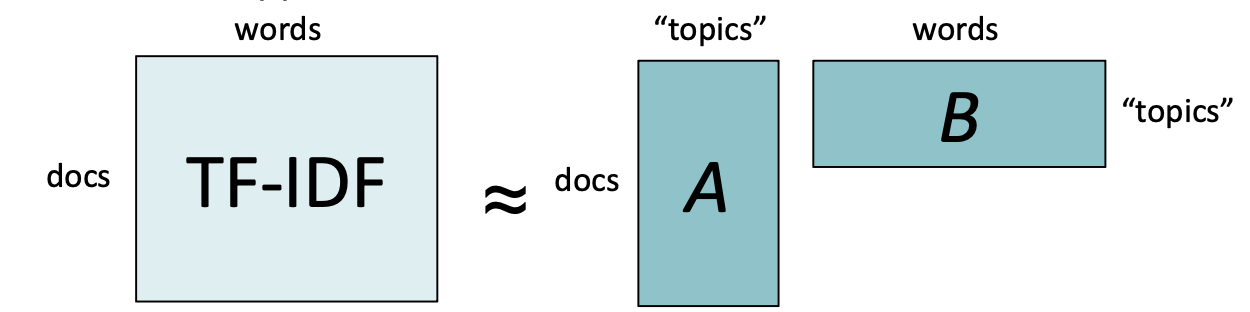
\includegraphics[width=0.8\textwidth]{matrix-factorization}
    \label{fig:LABEL}
\end{figure}

\begin{itemize}
	\item Assume docs and words have representation in (latent) "topic space"
	\item (IDF-weighted) word frequency modeled as dot products of doc's vectors and word's vectors in topic space
	\item \#topics $<<$ \#words ($\Rightarrow$ "dimensionality reduction"): D*W $\Rightarrow$ (D+W)*T
	\item Topics interpretable in doc space (A's cols) and word space (B's rows)
	\item Optimization problem: 
		\begin{itemize}
			\item Find \textit{A, B} such that \textit{AB} is as close to TF-IDF matrix as possible. That is, minimize 
			\begin{center}
				$\sum\limits_{d=1}^{N} \sum\limits_{w=1}^{M} (T_{dw} - A_d B_w)^{2}$
		\end{center}\\
		where \textit{T} is TF-IDF matrix, $A_d$ is \textit{d}-th row of \textit{A}, and $B_w$ is the \textit{w}-th column of \textit{B}
		\end{itemize}
	\item This is called \textbf{\textcolor{purple}{latent semantic analysis (LSA)}}
\end{itemize}

You already know how to efficiently compute this, from your linear algebra class: \textbf{\textcolor{orange}{singular-value decomposition}} (SVD)
\begin{itemize}
	\item $T = USV^{T}$, where \textit{U} and \textit{V} have columns that are orthogonal to each other (orthonormal bases), and \textit{S} is diagonal with in decreasing order. \textit{S} captures "importance" of topic (amount of variation in corpus w.r.t. topic)
	\item If you want \textit{k} topics, keep only the first \textit{k} columns of \textit{U} and \textit{V}, and the first \textit{k} rows and columns of \textit{S} $\Rightarrow$ \textit{U', S', V'}
	\item E.g., $A = U', B = S'V'^{T}$ or $A = U'S', B = V'^{T}$
\end{itemize}

Recall potential problem with clustering and classification and regression: "curse of dimensionality". \textbf{Matrix factorization} via \textbf{LSA} solves these problems for you: 
\begin{itemize}
	\item Use \textit{A} instead of original TF-IDF matrix
	\item That is, cluster (or learn to classify or regress) in topic space, rather than word space
\end{itemize}

Topic representation from LSA is simply a vector, not a probability distribution over topics. \textbf{Probabilistic}: LDA = Latent Dirichlet Allocation

\vspace{0.5cm}

\begin{center}
  {\LARGE \textbf{LDA: probabilistic topic modeling}}
\end{center}
\vspace{0.5cm}
\begin{itemize}
	\item Latent Dirichlet Allocation
	\item Document := bag of words
	\item Topic := probability distribution over words
	\item Each documents has a (latent) distribution over topics
	\item "Generative story" for generating a doc of length \textit{n}: \\
	d := sample a topic distribution for the doc ($\Leftarrow$ "Dirichlet") \\
	for \textit{i} = 1, ..., \textit{n} 

	\hspace{0.5cm} t := sample a topic from topic distribution \textit{d} 

	\hspace{0.5cm} w := sample a word from topic \textit{t} 

	\hspace{0.5cm}Add \textit{w} to the bag of words of the doc to be generated
\end{itemize}
This is \textbf{maximum-likelihood inference problem}! 

\section*{LDA example}

% Quick centered image
\begin{figure}[H]
    \centering
    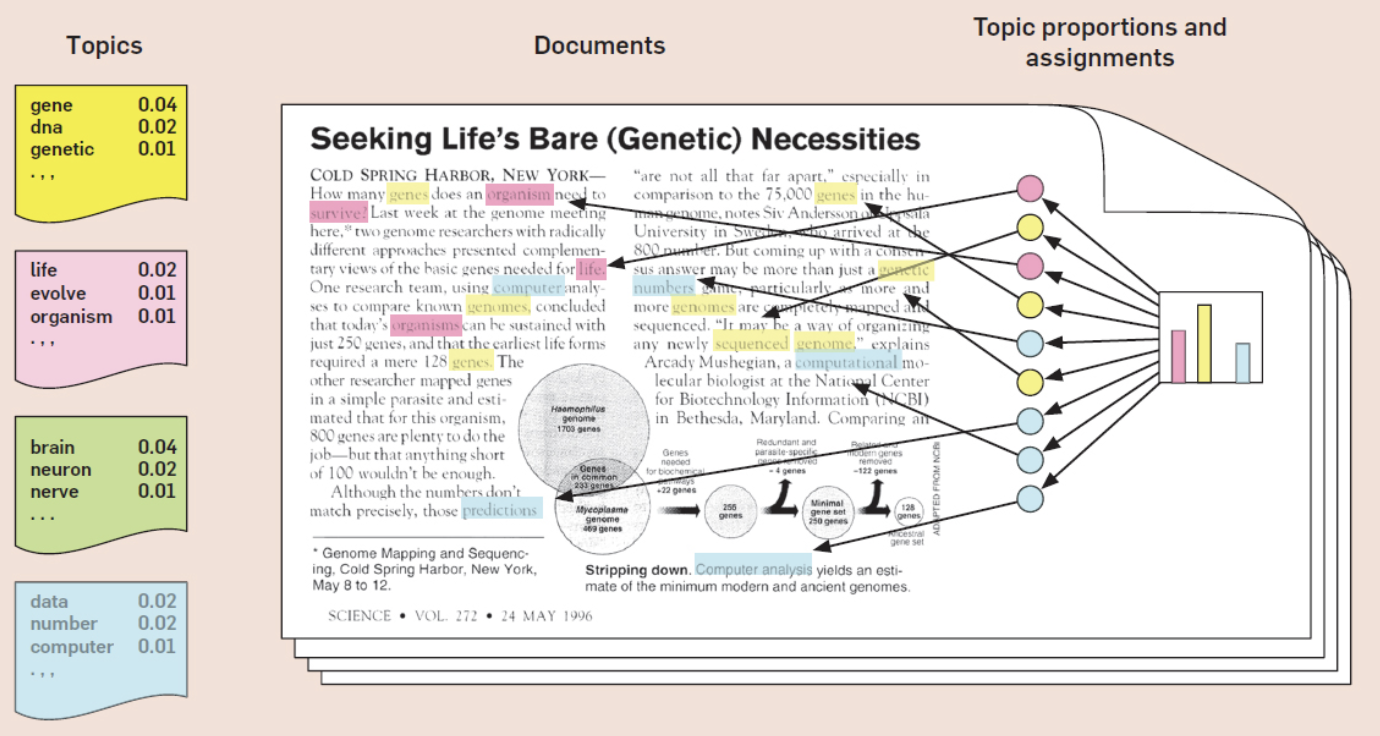
\includegraphics[width=1\textwidth]{LDA}
    \label{fig:LABEL}
\end{figure}

\begin{itemize}
	\item Each topic is represented as a distribution probability over words! We have, in order: \textbf{genetics}, \textbf{evolution}, \textbf{neuroscience} and \textbf{computer science}.
	\item The bar chart on the right is a categorical distribution over the select points. We can sample from this distribution all generated words! 
	\item LDA just gives the multi-set of words, not the order. The idea of LDA is to revert the above described process! 
\end{itemize}

\section*{Topic inference in LDA}
\begin{itemize}
	\item LDA is unsupervised (topics come out "magically")
	\item Input:
		\begin{itemize}
			\item Docs represented as bags of words
			\item Number \textit{K} of topics
		\end{itemize}
	\item Output:
		\begin{itemize}
			\item \textit{K} topics (distributions over words)
			\item For each doc: distribution over \textit{K} topics $\Rightarrow \theta_1$ = \{genetics: 0.3, evolution: 0.5, neuroscience: 0.2, computer science: 0\}
		\end{itemize}
	\item How is this done?
		\begin{itemize}
			\item Find distributions (i.e. topics, docs) that maximize the likelihood of the observed documents (maximum likelihood)
		\end{itemize}
\end{itemize}

\vspace{0.5cm}

\begin{center}
  {\LARGE \textbf{TF-IDF matrix}}
\end{center}
\vspace{0.5cm}

\section*{Question:}

\begin{itemize}
	\item "Which of these word pairs is more closely related?"
		\begin{itemize}
			\item (car, bus)
			\item (car, astronaut)
		\end{itemize}
	\item How to quantify this?
	\item Detour:
		\begin{itemize}
			\item How to quantify closeness of two docs?
			\item E.g., cosine of \textbf{rows} of TF-IDF matrix
			% Quick centered image
			\begin{figure}[H]
			    \centering
			    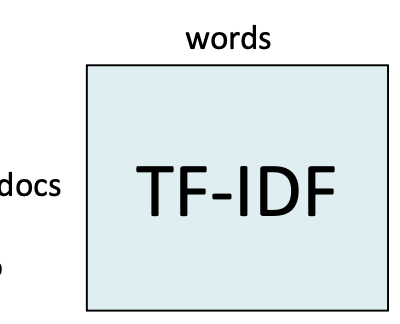
\includegraphics[width=0.2\textwidth]{TF-IDF}
			    \label{fig:LABEL}
			\end{figure}
		\end{itemize}
	\item Retour:
		\begin{itemize}
			\item How to quantify closeness of two words?
			\item E.g., cosine of \textbf{cols} of TF-IDF matrix. Cosine will be large if 2 words appears in the same set of documents! 
		\end{itemize}
\end{itemize}

\section*{Sparsity in TF-IDF matrix}
\begin{itemize}
	\item Two docs (i.e., rows of TD-IDF matrix)
		\begin{itemize}
			\item "Do you love men"?
			\item "Adorest thou the likes of Adam?"
			\item Cosine of row vectors of TF-IDF matrix == 0
		\end{itemize}
	\item Same problem when comparing two words (i.e., cols of matrix)
	\item Solution:
		\begin{itemize}
			\item Move from sparse to dense vectors. But how?
			\item Latent semantic analysis (LSA)! Use columns of \textit{B} as dense vectors representing words
			% Quick centered image
			\begin{figure}[H]
			    \centering
			    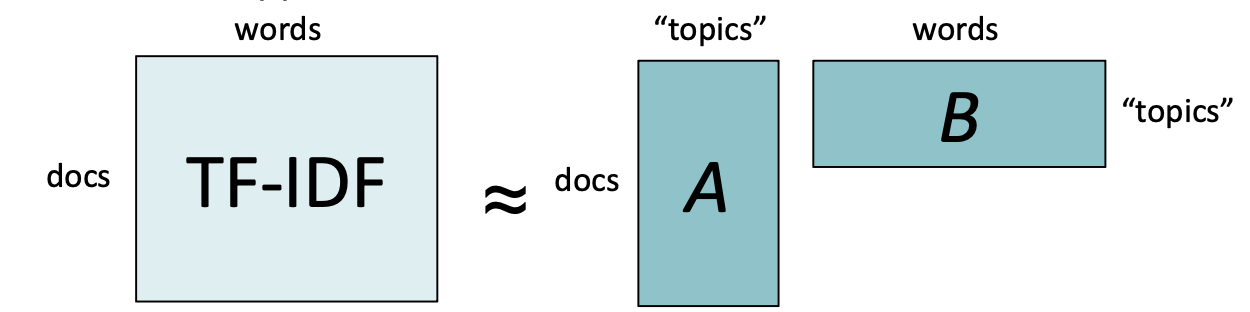
\includegraphics[width=0.4\textwidth]{matrix-factorization}
			    \label{fig:LABEL}
			\end{figure}
		\end{itemize}
\end{itemize}

\section*{"Word vectors"}
\begin{itemize}
	\item Idea: take into account how words appear together! Columns of TF-IDF matrix (sparse) or of word-by-topic matrix \textit{B} (dense), but all word representation is an entire doc treated as bag of words. All information about word proximity, syntax, etc., is lost.
	\item Solution: 
		\begin{itemize}
			\item Instead of full docs, consider local context: windows of \textit{L} (e.g., 3) consecutive words to \textcolor{blue}{left and right} of \textcolor{orange}{the target word}
			\item Rows of matrix: not docs, but contexts. 
			\item Pointwise mutual information(PMI):\\
				\textit{M}[\textit{c, w}] = PMI(\textit{c, w}) = $\log{\frac{Pr(c, w)}{Pr(c) \cdot Pr(w)}}$ \\
				"How much more likely are \textit{c} and \textit{w} to occur together than if they were independent?"
				% Quick centered image
				\begin{figure}[H]
				    \centering
				    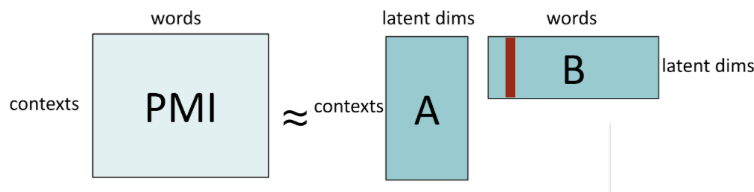
\includegraphics[width=0.8\textwidth]{context}
				    \label{fig:LABEL}
				\end{figure}
		\end{itemize}
	\item \underline{word2vec}: factor PMI matrix and use columns of \textit{B} as word vectors
\end{itemize}

\vspace{0.5cm}

\begin{center}
  {\LARGE \textbf{Beyond bags of words}}
\end{center}
\vspace{0.5cm}
\section*{From words to texts}

\begin{itemize}
	\item How to represent larger units, such as sentences, paragraphs, docs?
	\item Typical approach: take sum/average of words vectors
	\item Note: this is roughly also what bags of words are (when using "one-hot" encoding for words, i.e., vector with exactly one 1, rest 0)
	\item More recently: \textbf{learn} vectors for longer units
		\begin{itemize}
			\item Convolutional neural networks
			\item Recurrent neural networks: LSTM, ELMo
			\item Transformed-based models: \underline{BERT}, GPT-*
		\end{itemize}
\end{itemize}

\section*{BERT in a nutshell}
Introduced in 2018 by Google Research

% Quick centered image
\begin{figure}[H]
    \centering
    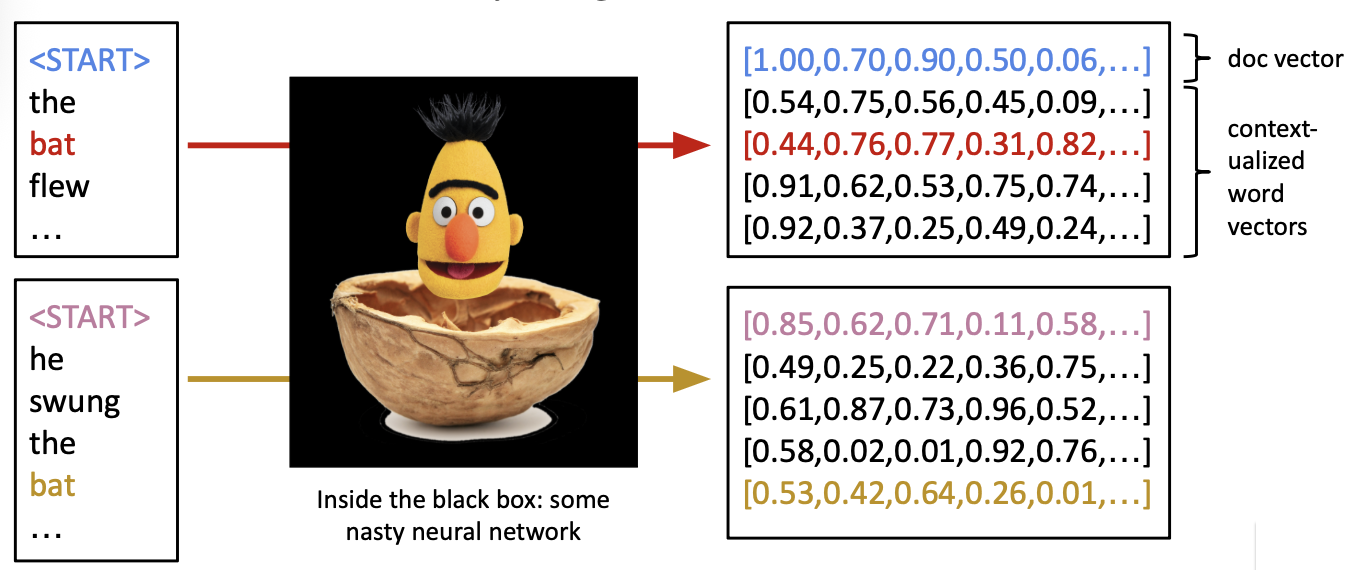
\includegraphics[width=0.8\textwidth]{bert}
    \label{fig:LABEL}
\end{figure}

\section*{NLP pipeline}
\begin{itemize}
	\item Tokenization
	\item Sentence splitting
	\item Part-of-speech (POS) tagging
	\item Named-entity recognition (NER)
	\item Coreference resolution
	\item Parsing
		\begin{itemize}
			\item Shallow parsing (a.k.a chunking)
			\item Constituency parsing
			\item Dependency parsing
		\end{itemize}
	\item \textbf{Sequential model}: fixed order of steps, early errors will propagate downstream. Fixer order not optimal for all cases...
	\item Hence, current research
	\item \textbf{Today's trend}: generative language models. 
\end{itemize}


\end{document}
